%% Преамбула TeX-файла

% 1. Стиль и язык
\documentclass[utf8x]{G7-32} % Стиль (по умолчанию будет 14pt)
\usepackage[T2A]{fontenc}
\usepackage[russian]{babel}
% Остальные стандартные настройки убраны в preamble.inc.tex.
\include{preamble.inc}

% Настройки листингов.
\include{listings.inc}

% Полезные макросы листингов.
% Любимые команды

\newtheorem{theorem}{Теорема}
\newtheorem{definition}{Определение}

\newcommand{\Code}[1]{\textbf{#1}}


\newcommand{\myImage}[3]{
\begin{figure}[!ht]
    \centering
    \includegraphics[width=\textwidth]{figures/#2}
    \caption{#1}
    \label{#3}
\end{figure}
}

\newcommand{\mySecondImage}[4]{
\begin{figure}[!ht]
    \centering
    \includegraphics[width=#4\textwidth]{figures/#2}
    \caption{#1}
    \label{#3}
\end{figure}
}


\begin{document}

\pagestyle{empty}
\begin{center}
    Министерство образования и науки Российской Федерации\\
    ФГАОУ ВПО  «УрФУ имени первого Президента России Б. Н. Ельцина»\\
    Институт радиоэлектроники и информационных технологий - РтФ\\
    Департамент информационных технологий и автоматики
    \par
    \vspace{4.5cm}
    \Large{
      WIFI-чип CC3100 и инструменты разработки

      \par
      \vspace{0.5cm}

      ОТЧЕТ\\
      по научно-исследовательской работе
    }

    \vspace{4cm}
    {
      Преподаватель: \hfill Ермакова Галина Михайловна
    }
    \par
    {
      Студент: \hfill Сухполюев Илья Владимирович
    }
    \par
    {
      Группа: \hfill РИ-440001
    }

    \par
    \vspace{3.5cm}
    Екатеринбург\\
    2017
\end{center}


\frontmatter % выключает нумерацию ВСЕГО; здесь начинаются ненумерованные главы: реферат, введение, глоссарий, сокращения и прочее.

% Команды \breakingbeforechapters и \nonbreakingbeforechapters
% управляют разрывом страницы перед главами.
% По-умолчанию страница разрывается.

% \nobreakingbeforechapters
% \breakingbeforechapters

% \include{00-abstract}
\pagestyle{plain}

\tableofcontents

% \include{10-defines}
% \include{11-abbrev}

\Introduction

Целью данной работы является изучение возможностей и
структуры wifi-чипа \textit{СС3100}\cite{cc3100}, разработанного и
поставляемого компанией \textit{Texas Instruments}, для использования
в качестве передатчика информации в рамках IoT-решений
(\textit{IoT -- Internet of Things -- Интернет вещей}).
Данное исследование является предварительным сбором сведений
для возможной интеграции чипа с миниатюрными диктофонами
ООО <<Вторая лаборатория>>\cite{labi2dicts}, с целью
осуществления удаленной настройки диктофона и получения
уже записанных аудиоданных c диктофона. Поэтому одними
из главных исследуемых характеристик будет пропускная способность
и низкое энергопотребление, как при работе чипа, так и при
выключенном (спящем) режиме.

Чип CC3100 создан для предоставления готового стека
Интернет протоколов на устройства с отдельным модулем управления
\textit{MCU} (\textit{Microcontroller Unit}), поэтому для
проведения требуемых измерений помимо самого чипа
требуется установка, позволяющая предоставить
требуемое питание и задающая внешнее программное управление.
Для этих целей компания Texas Instruments поставляет
установки \textit{CC3100BOOST}\cite{cc3100boost} и \textit{CC31XXEMUBOOST}\cite{cc31xxemuboost},
а также прилагает к ним программные инструменты для разработки
\textit{SDK}(\textit{Software Development Kit}) для запуска
отладочных управляющих программ на стационарном компьютере,
которые могут помочь в тестировании заявленных чипом CC3100
характеристик.

\clearpage
Таким образом, для достижения поставленной цели необходимо решить следующие задачи:

\begin{itemize}
\item Изучить документацию и рекомендации по разработке, прилагающееся к CC3100;
\item Ознакомиться с устройством и документацией схемы CC3100BOOST;
\item Ознакомиться с устройством и документацией схемы CC31XXEMUBOOST;
\item Собрать на основе схем CC3100BOOST и CC31XXEMUBOOST отладочную установку;
\item Запустить на полученной установке примеры программ из СС3100SDK;
\item Провести тестирование пропускной способности CC3100, используя рассмотренные примеры
программ и руководства к разработке.
\end{itemize}


\mainmatter % это включает нумерацию глав и секций в документе ниже

\chapter{Обзор документации к исследуемым устройствам}
\label{cha:analysis}
%
% % В начале раздела  можно напомнить его цель
%

\myImage{cc3100-docs}{cc3100-docs}{cc3100-docs}


\section{CC3100}
\cite{cc3100datasheet}
\cite{cc3100userguide}
\cite{cc3100wiki}


\mySecondImage{cc3100-logic-structure}{cc3100-logic-structure}{cc3100-logic-structure}{0.5}
\mySecondImage{cc3100-internet-stack}{cc3100-internet-stack}{cc3100-internet-stack}{0.5}
\myImage{cc3100-spi-timing}{cc3100-spi-timing}{cc3100-spi-timing}
\mySecondImage{cc3100-spi-flash}{cc3100-spi-flash}{cc3100-spi-flash}{0.6}
\mySecondImage{cc3100-spi-mcu}{cc3100-spi-mcu}{cc3100-spi-mcu}{0.6}

\myImage{cc3100-state-machine}{cc3100-state-machine}{cc3100-state-machine}

\section{CC3100BOOST \& CC31XXEMUBOOST}

\mySecondImage{boost-logic-scheme}{boost-logic-scheme}{boost-logic-scheme}{0.7}
\myImage{boost-pins}{boost-pins}{boost-pins}




%%% Local Variables:
%%% mode: latex
%%% TeX-master: "rpz"
%%% End:

\chapter{CC3100SDK}
\label{cha:design}

\section{Получение SDK}

\section{Внутреннее устройство SDK}

\section{Примеры управляющих программ}

\subsection{Программа 1}

\subsection{Программа 2}


%%% Local Variables:
%%% mode: latex
%%% TeX-master: "rpz"
%%% End:

\chapter{Тестирование пропускной способности CC3100}
\label{cha:impl}


\begin{verbatim}
int main(int argscount, char *args[])
{
    if(argscount < 3) {
        fprintf(stderr, 'not enough arguments\n');
        exit(-1);
    }

    setUP_and_check();

    uint64_t len = (uint64_t)atoi(args[1]);
    const char * filename = args[2];
    DEBUG("Read file: %s, filesize: %d", filename, len);
    FILE* f = fopen(filename, "rb");
    void* data = malloc(len);
    fread(data, 1, len, f);
    close(f);
    DEBUG("data has been read");

    int32_t sockId = sl_Socket(SL_AF_INET, SL_SOCK_STREAM, SL_IPPROTO_TCP);
    assert(sockId >= 0);

    SlSockAddrIn_t addr = {
            .sin_family = SL_AF_INET,
            .sin_port = sl_Htons(8080),
            .sin_addr.s_addr = sl_Htonl(
                    // 0xC0A80064 // 192.168.0.100
                    0xC0A80067 // 192.168.0.103
                    // 0xC0A82B48 // 192.168.43.72
                    ),
    };
    int16_t status = sl_Connect(sockId, (SlSockAddr_t *) &addr, sizeof(SlSockAddrIn_t));
    assert(status >= 0);
    DEBUG("connected");

    for(int32_t i = 0; i < len / 1024; i++) {
            status = sl_Send(sockId, data + i * 1024, 1024, 0);
            assert(status > 0);
    }
    sl_Close(sockId);

    DEBUG("data sended");
    return 0;
}
\end{verbatim}

\begin{verbatim}
def start_server():
    server = socket.socket(socket.AF_INET, socket.SOCK_STREAM)
    server.bind(('0.0.0.0', 8080))
    server.listen()
    print('[server] start listening', file=sys.stderr)
    (client, address) = server.accept()  # : :type client: socket.socket
    print('[server][%s:%d] get connectinon.' % address, file=sys.stderr)
    start = time.time()

    data = []
    recived_bytes = 0
    while True:
        part = client.recv(4096)
        if part == b'':
            break
        recived_bytes += len(part)
        data.append(part)

    end = time.time()
    client.close()
    print('[server][%s:%d] close connection. Recievd %f Mb; Time: %f' % (
        address[0], address[1], recived_bytes / (1024 * 1024), end - start),
        file=sys.stderr)

    return (data, recived_bytes / (1024 * 1024), end - start)
\end{verbatim}

\myImage{bandwidth-test}{bandwidth-test}{bandwidth-test}

%%% Local Variables:
%%% mode: latex
%%% TeX-master: "rpz"
%%% End:

% \include{50-research}

\backmatter %% Здесь заканчивается нумерованная часть документа и начинаются ссылки и
            %% заключение

\include{80-conclusion}

\include{81-biblio}

\appendix   % Тут идут приложения

\chapter{Изображения устройств}
\label{cha:appendix1}

\begin{figure}[!ht]
    \centering
    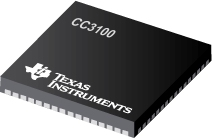
\includegraphics[width=0.5\textwidth]{figures/CC3100}
    \caption{Wifi-чип CC3100}
    \label{apx:cc3100}
\end{figure}

\begin{figure}[!ht]
    \centering
    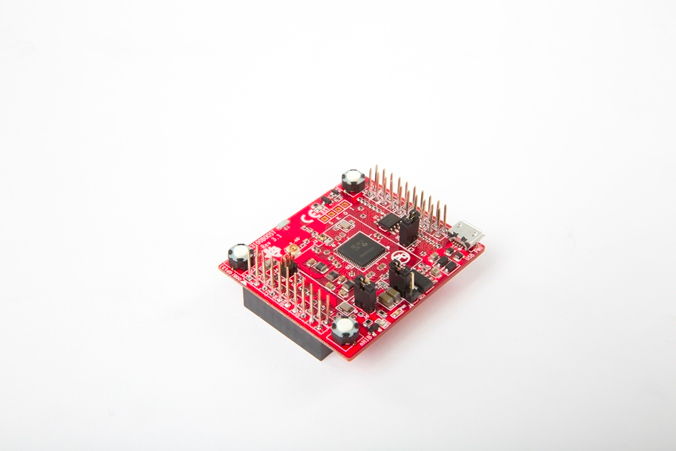
\includegraphics[width=\textwidth]{figures/CC3100BOOST}
    \caption{CC3100BOOST -- отладочная установка}
    \label{apx:cc3100boost}
\end{figure}

\begin{figure}[!ht]
    \centering
    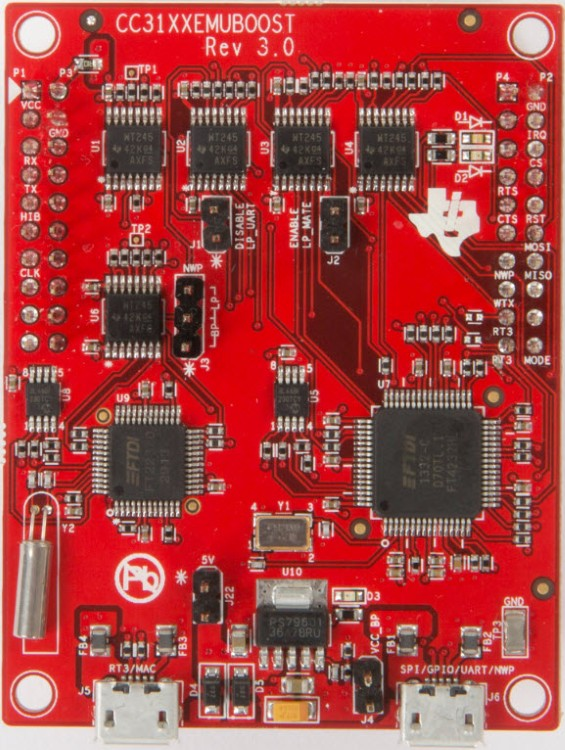
\includegraphics[width=0.6\textwidth]{figures/CC31XXEMUBOOST}
    \caption{CC31XXEMUBOOST -- установка для предоставления управления
    ПК через USB порт}
    \label{apx:cc31xxemuboost}
\end{figure}

%%% Local Variables:
%%% mode: latex
%%% TeX-master: "rpz"
%%% End:

\chapter{Исходный код программ}
\label{cha:appendix2}



\section{Тестирование пропускной способности}

\begin{verbatim}
#!/usr/bin/env python
import argparse
import socket
import sys
import time


def parse_args():
    parser = argparse.ArgumentParser()
    parser.add_argument('-f', '--filename', type=str, required=True)
    return parser.parse_args()


def start_server():
    server = socket.socket(socket.AF_INET, socket.SOCK_STREAM)
    server.bind(('0.0.0.0', 8080))
    server.listen()
    print('[server] start listening', file=sys.stderr)
    (client, address) = server.accept()  # : :type client: socket.socket
    print('[server][%s:%d] get connectinon.' % address, file=sys.stderr)
    start = time.time()

    data = []
    recived_bytes = 0
    while True:
        part = client.recv(4096)
        if part == b'':
            break
        recived_bytes += len(part)
        data.append(part)

    end = time.time()
    client.close()
    print('[server][%s:%d] close connection. Recievd %f Mb; Time: %f' % (
        address[0], address[1], recived_bytes / (1024 * 1024), end - start),
        file=sys.stderr)

    return (data, recived_bytes / (1024 * 1024), end - start)


def check_data(data, src_filename):
    with open(src_filename, mode='rb') as file:
        for part in data:
            origin_part = file.read(len(part))
            if part != origin_part:
                print('[server][ERROR] Data check is faild.', file=sys.stderr)
                sys.exit(status=-1)
    print('[server] Data check is passed.', file=sys.stderr)


def main():
    args = parse_args()
    (data, size, recv_time) = start_server()
    check_data(data, args.filename)
    print(size, recv_time)


if __name__ == '__main__':
    main()
\end{verbatim}


\begin{verbatim}
#include "header.h"


void setUP_and_check() {
        int32_t retVal = configureSimpleLinkToDefaultState(defaultDevName());
        if(retVal < 0) {
                DEBUG("Failed to configure in default state; Error: %ld", retVal);
                exit(-1);
        }
        DEBUG("Device is configured in default state");

        retVal = sl_Start(0, defaultDevName(), 0);
        if (retVal < 0 || ROLE_STA != retVal) {
                DEBUG("Failed to start the device; Error: %ld", retVal);
                exit(-1);
        }
        DEBUG("Device started as STATION");

        retVal = connectToAP("labi2", SL_SEC_TYPE_WPA_WPA2, "labi2_wpa");
        if(retVal < 0) {
                DEBUG("Failed to establish connection with AP; Error: %ld", retVal);
                exit(-1);
        }
        DEBUG("Connection established with AP and IP is acquired");

        DEBUG("Checking LAN connection - pinging Gateway...!");
        retVal = pingTargetHost(g_GatewayIP);
        if(retVal < 0) {
                DEBUG("Device couldn't connect to LAN; Error: %ld", retVal);
                exit(-1);
        }
        DEBUG("Device successfully connected");
}


int main(int argscount, char *args[])
{
        if(argscount < 3) {
                fprintf(stderr, 'not enough arguments\n');
                exit(-1);
        }

        setUP_and_check();

        uint64_t len = (uint64_t)atoi(args[1]);
        const char * filename = args[2];
        DEBUG("Read file: %s, filesize: %d", filename, len);
        FILE* f = fopen(filename, "rb");
        void* data = malloc(len);
        fread(data, 1, len, f);
        close(f);
        DEBUG("data has been read");

        int32_t sockId = sl_Socket(SL_AF_INET, SL_SOCK_STREAM, SL_IPPROTO_TCP);
        assert(sockId >= 0);

        SlSockAddrIn_t addr = {
                .sin_family = SL_AF_INET,
                .sin_port = sl_Htons(8080),
                .sin_addr.s_addr = sl_Htonl(
                        // 0xC0A80064 // 192.168.0.100
                        0xC0A80067 // 192.168.0.103
                        // 0xC0A82B48 // 192.168.43.72
                        ),
        };
        int16_t status = sl_Connect(sockId, (SlSockAddr_t *) &addr, sizeof(SlSockAddrIn_t));
        assert(status >= 0);
        DEBUG("connected");

        for(int32_t i = 0; i < len / 1024; i++) {
                status = sl_Send(sockId, data + i * 1024, 1024, 0);
                assert(status > 0);
        }
        sl_Close(sockId);

        DEBUG("data sended");
        return 0;
}
\end{verbatim}

%%% Local Variables:
%%% mode: latex
%%% TeX-master: "rpz"
%%% End:


\end{document}

%%% Local Variables:
%%% mode: latex
%%% TeX-master: t
%%% End:
